\documentclass{article}
\usepackage{amsmath, amssymb, tikz, marvosym, tcolorbox, array, sfmath, enumerate, pgfplots, multicol, framed}
\usepackage[hidelinks]{hyperref}
\renewcommand{\familydefault}{\sfdefault}
\pgfplotsset{compat=newest}
\usetikzlibrary{arrows.meta}
\everymath{\displaystyle}
\tikzset{>=stealth}
\tikzstyle{input} = [circle, text centered, radius = 1cm, draw = black]
\tikzstyle{function} = [rectangle, text centered, minimum width = 2cm, minimum height = 1cm, draw = black]
\usepackage[top = 0.25in, bottom = 0.25in, left = 1in, right = 1in]{geometry}
\pagestyle{empty}
\raggedright

\newcounter{example}[section]
\newenvironment{example}[1][]{\refstepcounter{example}\par\medskip
   {\color{red}\textbf{Example~\theexample. #1}}}{\medskip}
\usepackage{hyperref}
\begin{document}

\section*{Intro to Functions}

\begin{tcolorbox}[colframe=orange!70!white, coltitle=black, title=\textbf{Summary}]
\begin{enumerate}
    \item A function has only one output value for each input value.
    \item Function notation can be used to describe and quickly evaluate a function.
\end{enumerate}
\end{tcolorbox}
\bigskip 

\subsection*{Relations and Functions}


\begin{tcolorbox}[colframe=green!80!blue, coltitle=white, title=\textbf{Relations}]
A \textbf{relation} is a set of ordered pairs.
\end{tcolorbox}
\bigskip  

\begin{tcolorbox}[colframe=green!80!blue, coltitle=white, title=\textbf{Domain}]
The \textbf{domain} is the set of all input values (usually $x$) of a relation.
\end{tcolorbox}
\bigskip  

\begin{tcolorbox}[colframe=green!80!blue, coltitle=white, title=\textbf{Range}]
The \textbf{range} is the set of all output values (usually $y$) of a relation.
\end{tcolorbox}
\bigskip 

\begin{tcolorbox}[colframe=green!80!blue, coltitle=white, title=\textbf{Function}]
A \textbf{function} is a relation is which each element of the domain has only 1 element in the range.
\end{tcolorbox}
\bigskip  
% \newpage

\begin{example} 
Determine whether each relation represents a function. \\
For those that do, state the domain and range.
\begin{enumerate}[(a)]
\begin{multicols}{2}
    \item $\{(1,5), \, (2, 5), \, (3, 7), \, (4, 8)\}$ \label{ex1a}
    \item $\{(5,1), \, (5,2), \, (7,3), \, (8,4)\}$ \label{ex1b}
\end{multicols}
\end{enumerate}
\end{example}
\vfill 

\subsection*{The Vertical Line Test}
It is also possible to determine if a relation is a function visually by using the {\color{blue}\textbf{vertical line test}}:
\bigskip 

\begin{tcolorbox}[colframe=green!80!blue, coltitle=white, title=\textbf{Vertical Line Test}]
If every vertical line drawn hits the graph \underline{\textbf{at most once}}, then the relation is a function.
\end{tcolorbox}
\vspace{0.25in} 
\newpage

\begin{minipage}{0.5\textwidth}
\textsc{\href{ex1a}{Example 1\ref{ex1a}} Passes V.L.T.}
\begin{center}
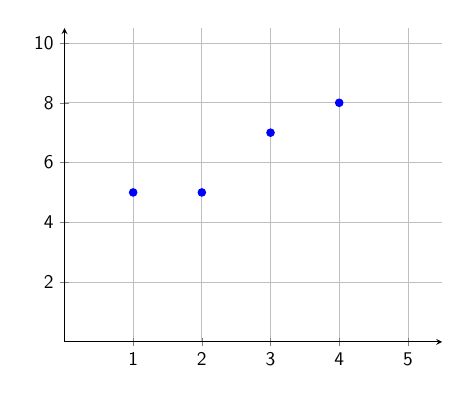
\begin{tikzpicture}[scale=0.7]
\begin{axis}[
	axis lines = middle,
	grid=both,
	xmin = 0, xmax = 5.5,
	ymin = 0, ymax = 10.5
]
\addplot[color=blue, mark = *, only marks] coordinates {(1,5) (2,5) (3,7) (4,8)};
\end{axis}
\end{tikzpicture}
\end{center}
\end{minipage}
\begin{minipage}{0.45\textwidth}
\textsc{\href{ex1b}{Example 1\ref{ex1b}} Fails V.L.T.}
\begin{center}
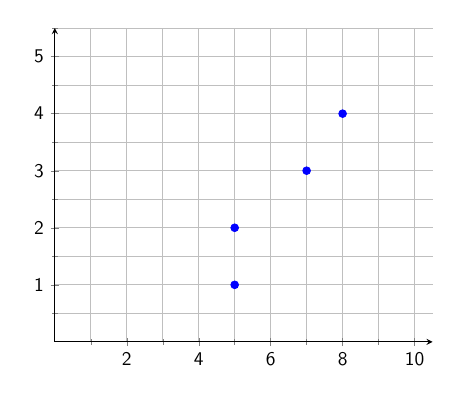
\begin{tikzpicture}[scale=0.7]
\begin{axis}[
	axis lines = middle,
	grid=both, minor tick num = 1,
	xmin = 0, xmax = 10.5,
	ymin = 0, ymax = 5.5
]
\addplot[color=blue, mark = *, only marks] coordinates {(5,1) (5,2) (7,3) (8,4)};
\end{axis}
\end{tikzpicture}
\end{center}
\end{minipage}
\vfill 

\begin{example}
Determine whether the graph of each represents a function.
\begin{enumerate}[(a)]
\begin{multicols}{3}
    \item \mbox{} \newline\\
    \begin{tikzpicture}[domain = -1.5:1.5]
	\draw [<->] (-2,0) -- (2,0);
	\node at (2,0) [anchor = west] {\tiny $x$};
	\draw [<->] (0,-2) -- (0,2);
	\node at (0,2) [anchor = west] {\tiny $y$};
	\draw [<->, color = blue, very thick] plot(\x, {-1/2*\x-1/2});
    \end{tikzpicture}
    
    \item \mbox{} \newline\\
    \begin{tikzpicture}[domain = -1.5:1.5]
	\draw [<->] (-2,0) -- (2,0);
	\node at (2,0) [anchor = west] {\tiny $x$};
	\draw [<->] (0,-2) -- (0,2);
	\node at (0,2) [anchor = west] {\tiny $y$};
	\draw [<->, color = blue, very thick] plot(\x, {-1/2*\x*\x+1/2});
    \end{tikzpicture}
    
    \item \mbox{} \newline\\
    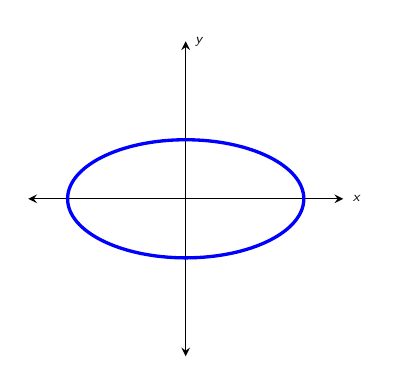
\begin{tikzpicture}
	\draw [<->] (-2,0) -- (2,0);
	\node at (2,0) [anchor = west] {\tiny $x$};
	\draw [<->] (0,-2) -- (0,2);
	\node at (0,2) [anchor = west] {\tiny $y$};
	\draw [color = blue, very thick] (0,0) ellipse (1.5 and 0.75);
    \end{tikzpicture}
\end{multicols}
\end{enumerate}
\end{example}
\vfill 
\newpage 
    
\subsection*{Function Notation.}

Think of a function as a \textbf{machine}. 
\bigskip 

You give the function (machine) a value (input), \newline 
it will process that value, and then return a value back to you (output).
\bigskip 

For instance, if you input 10 into the $x^2$ function, it will return $10^2$, or 100:	\newline\\

\begin{center}
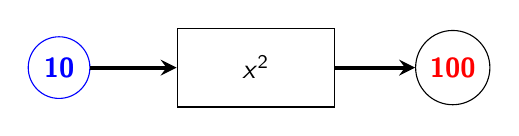
\begin{tikzpicture}[node distance = 2.5 cm]
\node (inputVal) [input, color=blue] {\color{blue}\textbf{10}};
\node (func) [function, right of = inputVal] {$x^2$};
\node (outputVal) [input, right of = func] {\color{red}\textbf{100}};

\draw [->, >=stealth, thick, line width = 1.5] (inputVal) -- (func);
\draw [->, >=stealth, thick, line width = 1.5] (func) -- (outputVal);
\end{tikzpicture}
\end{center}
\vspace{0.25in}

A function can be described using \textbf{function notation}. 
\bigskip 

\begin{center}
\begin{framed}
$f(x)$ represents the value of the function when the value of $x$ is substituted into it.
\end{framed}
\end{center}
\bigskip 

We can use other notations for functions including, but not limited to,
\[ g(x) \quad h(x) \quad f(n) \quad f\left(\text{\Smiley}\right) \]
\bigskip 

When we substitute a value for the variable and evaluate it, that is called {\color{blue}\textbf{evaluating the function}}. \newline\\

For the $f(x) = x^2$ function, the point (10, 100) is on the graph of that function.
\bigskip 

\begin{example}
Evaluate $f(2), \, f(-2), \, \text{and } f(0)$ for each.
\begin{enumerate}[(a)]
\begin{multicols}{2}
    \item $f(x) = 2x + 3$
    \item $f(x) = 3x^2-1$ 
\end{multicols}
\vfill 

\begin{multicols}{2}
    \item \mbox{} \newline\\
    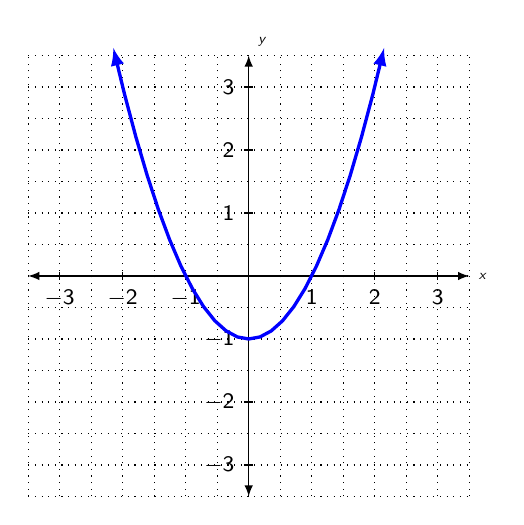
\begin{tikzpicture}[domain = -2.15:2.15, scale=0.8]
	\draw [step = 0.5cm, dotted] (-3.5,-3.5) grid (3.5,3.5);
	\draw[<->, > = latex] (-3.5,0) -- (3.5,0);
	\node at (3.5,0) [anchor = west] {\tiny $x$};
	\draw[<->, > = latex] (0,-3.5) -- (0,3.5);
	\node at (0,3.5) [anchor = south west] {\tiny $y$};
	\foreach \x in {-3,-2,-1,1,2,3}
	\draw[shift = {(\x,0)}] (0pt,2pt) -- (0pt, -2pt) node[below] {\footnotesize $\x$};
	\foreach \y in {-3,-2, -1, 1, 2, 3}
	\draw[shift = {(0,\y)}] (2pt,0pt) -- (-2pt,0pt) node[left] {\footnotesize $\y$};
	\draw [<->, > = latex, color = blue, very thick]	plot (\x, {\x*\x - 1});
    \end{tikzpicture}

    \item \mbox{} \newline\\
    \begin{tabular}{|c|c|c|c|c|c|c|c|}
        $x$ & $-3$ & $-2$ & $-1$ & 0 & 1 & 2 & 3 \\ \hline
        $f(x)$ & $-6$ & 3 & 4 & $-3$ & $-8$ & 6 & $-5$ \\
    \end{tabular}
\end{multicols}
\end{enumerate}
\end{example}

\vspace{0.25in} 

\newpage 

\subsection*{Building Functions}

We can build functions according to specifications listed. 
\bigskip 

\begin{example}
Build a function, $f(x)$, that will perform each of the following sequences of instructions.
\begin{enumerate}[(a)]
    \item 
        \begin{enumerate}[1.]
            \item Add 5 to the input    \\[0.5in]
            \item Take half of that result
    \end{enumerate}
    \vfill 
    \item 
        \begin{enumerate}[1.]
            \item Take half of the input    \\[0.5in]
            \item Add 5 to that result
        \end{enumerate}
    \vfill 
    \item
        \begin{enumerate}[1.]
            \item Take the opposite of the input    \\[0.5in]
            \item Subtract 9 from that result   \\[0.5in]
            \item Multiply that result by $-2$  \\[0.5in]
        \end{enumerate}
    \vfill 
\end{enumerate}
\end{example}

\end{document}
